
\begin{figure}[H]
  \centering
  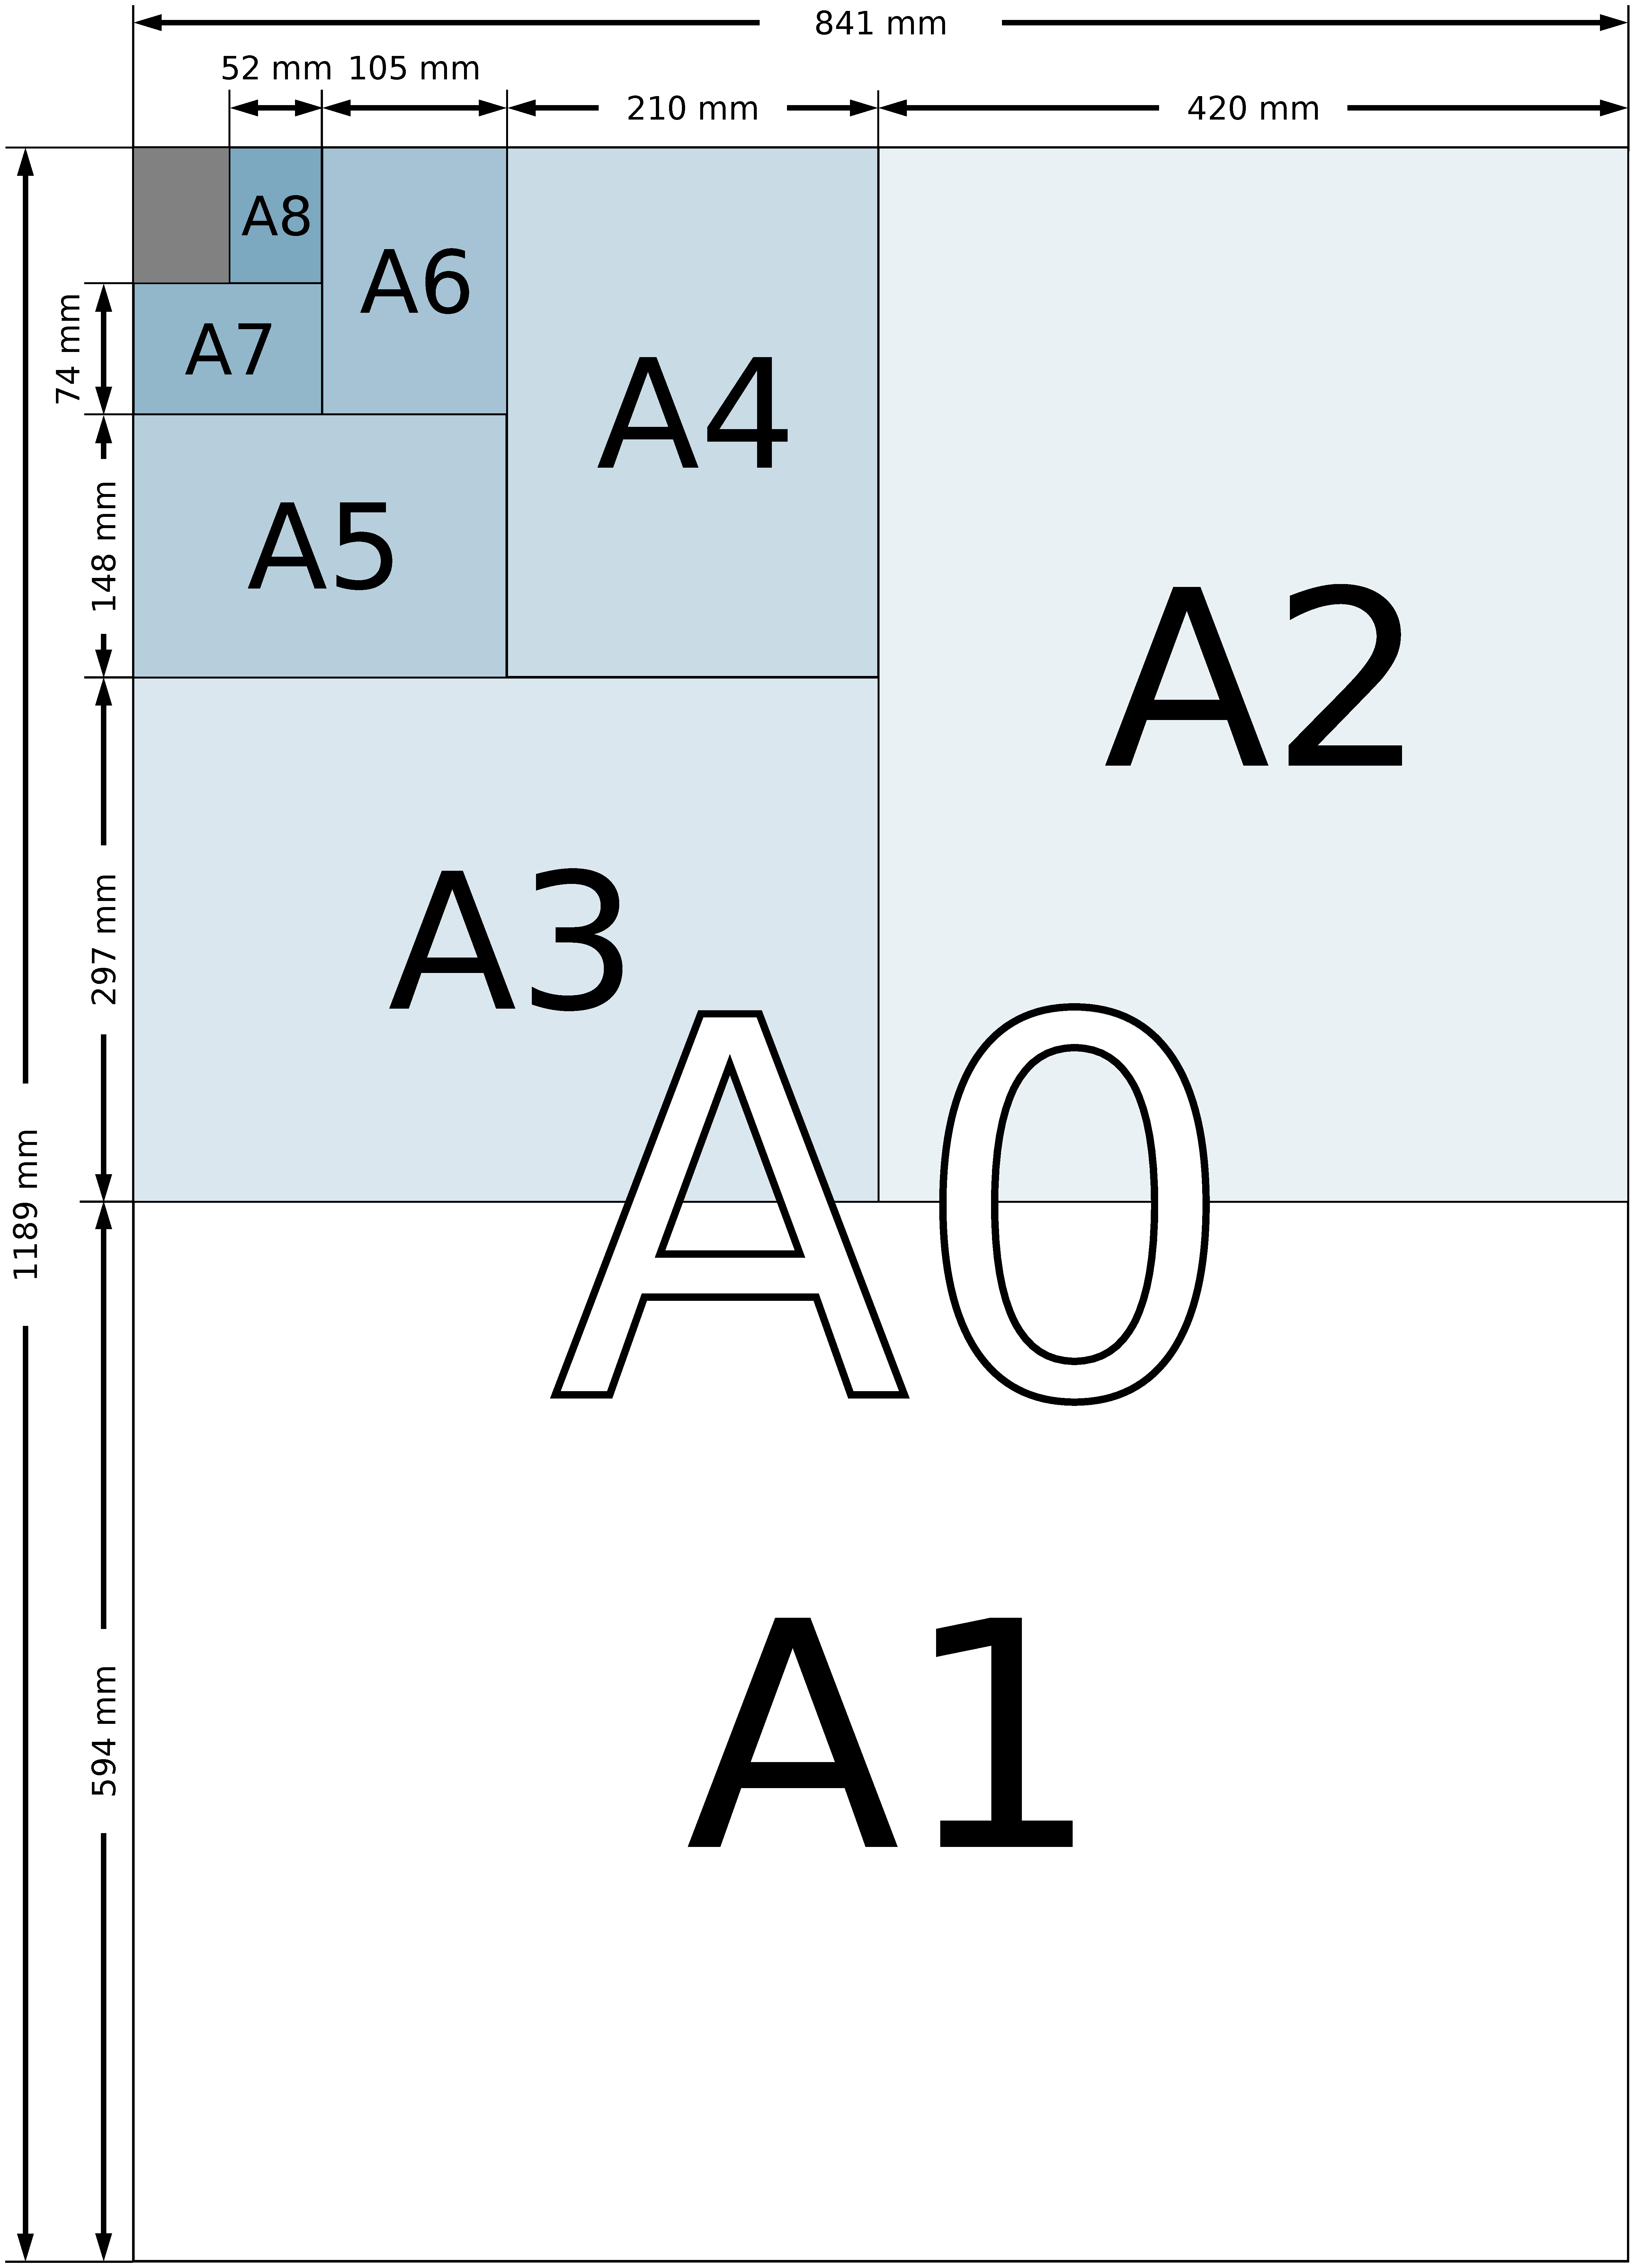
\includegraphics[angle=270,origin=c,width=0.8\textwidth]{includes/A-paper-eps}
\end{figure}

\section*{Introduction}
Understanding the properties of arithmetic and geometric sequences are essential for quantifying the world, and for computing in general. In this paper, I will investigate the different sizes of ISO 216 standard A-series paper, and quantify their properties using my knowledge of sequences.

\section*{The Properties of ISO 216 A-Series Paper}
Let us begin by quantifying the properties of ISO 216 A-series paper (henceforth referred to as A-paper). It is given that the largest A-paper size, $A_{0}$, has a total area of \SI{1}{\metre\squared}. Likewise, we know that each successive smaller paper is the previous paper folded in half.

\subsection*{Formalising the Area}
We can formalise this property as the following geometric sequence:

\begin{align*}
  a_{n} &= a \times r^{n - 1} \\
  A_{n} &= A \times \left(\frac{1}{2}\right)^{n -1} \\
        &= 2^{-n}
\end{align*}

\noindent
By plugging in the the numbers, it is trivial to generate a table of area for each successive A-series paper:

\begin{table}[h]
  \centering\makegapedcells
    \begin{tabular}{@{}lcl@{}}
    \toprule
    $n$ & Area (fractional \si{\meter\squared}) & Area (decimal \si{\meter\squared}) \\ \midrule
    $0$ & $1$               & $1$              \\
    $1$ & $\frac{1}{2}$     & $0.5$            \\
    $2$ & $\frac{1}{4}$     & $0.25$           \\
    $3$ & $\frac{1}{8}$     & $0.125$          \\
    $4$ & $\frac{1}{16}$    & $0.0625$         \\
    $5$ & $\frac{1}{32}$    & $0.03125$        \\
    $6$ & $\frac{1}{64}$    & $0.015625$       \\ \bottomrule
  \end{tabular}
  \caption{List of A-series paper areas for $0 \geq n \leq 6$}
  \label{tab:area}
\end{table}

\subsection*{Formalizing the Length and Width}
The geometric sequence behind the area of the A-series paper is trivial to discover, but what about the length and width of the paper for a given $n$ in $A_{n}$? Recall that every time an A-series paper is folded in half, we make the fold at the largest side (the length) of the paper:

\begin{align*}
  A_{n}     &= L_{n} \times W_{n} \\
  A_{n + 1} &= \frac{L_{n}}{2} \times W_{n}
\end{align*}

\noindent
Where essentially the new "length" of $A_{n + 1}$ is actually the width of the previous larger paper, namely $A_{n}$:

\begin{align*}
  L_{n + 1} &= W_{n} \\
  W_{n + 1} &= \frac{L_{n}}{2}
\end{align*}

\noindent
This relation is apparent even if we just list out the sequences:

\[
  \begin{array}{*{8}{l@{\ }}}
    L_{n} = & L_{0}, & \frac{L_0}{2}, & \frac{L_{0}}{2}, & \frac{L_{0}}{4}, & \frac{L_{0}}{4}, & \frac{L_{0}}{8}, & \frac{L_{0}}{8}, \\[\jot]
    W_{n} = & W_{0}, &         W_{0}, & \frac{W_{0}}{2}, & \frac{W_{0}}{2}, & \frac{W_{0}}{4}, & \frac{W_{0}}{4}, & \frac{W_{0}}{8},
  \end{array}
\]

\noindent
This property is an important one, because it allows us to discover the ratio, or \emph{aspect ratio} between the two sides of the paper. We must do this prior to the next section on the scaling factor, because without knowing the aspect ratio of the sides, there is no way for us to do proper scaling conversions. Hence, let $R_{n}$ be the aspect ratio of $A_{n}$

\begin{align*}
  R_{n}     &= \frac{L_{n}}{W_{n}} \\
  R_{n + 1} &= \frac{L_{n + 1}}{W_{n + 1}} \\
            &= \frac{W_{n}}{L_{n} \div 2} \\
            &= \frac{2W_{n}}{L_{n}} \\
            &= \frac{2}{L_{n} \div W_{n}}
\end{align*}

\noindent
Originally, I hoped that somehow the terms would cancel out and I would be able to have a numerical solution, but that didn't happen. However, not all was lost, because in the process of working out this math I came to another realisation. Now recall that we defined $R_{n}$ as $\frac{L_{n}}{W_{n}}$. Therefore:

\begin{align*}
  R_{n + 1} &= \frac{2}{L_{n} \div W_{n}} \\
            &= \frac{2}{R_{n}}
\end{align*}

\noindent
Do you recall how in the Lecture, we were told that one of the properties of the A-series paper, was how each time you fold it in half it preserves the proportions of the previous paper? This is a property that is unique to the ISO 216 paper, if you take a U.S. Letter paper and fold it in half, every time you fold it you end up with a slightly different rectangle. Now, there is only one way that this property can happen --- namely that the aspect ratio of each subsequent halve must be the same, e.g $R_{n} = R_{n + 1} = R_{n + 2}$ for $n \to \infty$. Therefore:

\begin{align*}
  R_{n + 1} &= \frac{2}{R_{n}} = R_{n}
\end{align*}

\noindent
Now we have the simple numerical solution that I was looking for! We can find the value of $R_{n}$ simply by solving for it:

\begin{align*}
  R_{n} &= \frac{2}{R_{n}} \\
  R_{n} \times R_{n} &= 2 \\
  \left(R_{n}\right)^2 &= 2 \\
  R_{n} &= \sqrt{2}
\end{align*}

\noindent
Now that we found the aspect ratio, generating a sequence of lengths and widths becomes a trivial process involving the aspect ratio, where $L:W::1:\sqrt{2}$. I will demonstrate the work here:

\begin{align*}
  A_{n} &= L_{n} \times W_{n} = 1 \\
      1 &= L_{n} \times \left(L_{n} \times \frac{1}{\sqrt{2}}\right) \\
      1 &= \frac{\left(L_{n}\right)^2}{\sqrt{2}} \\
  \frac{1}{\sqrt{2}} &= \left(L_{n}\right)^2 \\
  \frac{1}{2} &= L_{n}
\end{align*}

\subsection*{The Scaling Factor of Conversions}
